%-----------------------------------------------------------------------
\chapter{Previous Work}
\label{sec:previous}

%-----------------------------------------------------------------------
\section{Facial Animation} \label{sec:prfacialanimation}

The first attempts at using performance-driven facial animation in academia date back to late $20^{th}$ century while in industry it was first used for guidance rather than production, for instance the facial motion of Gollum in the \textit{Lord of the Rings} was based on the motion capture data of the performance of the role actor Andy Serkis~\cite{Pighin:2002}. Another notable example is the pipeline used in the making of \textit{the Polar Express}; the motion capture data was used to construct a multilayer facial rig that was used by an artist to create the final facial animation~\cite{Bennett:2005}. Though many other examples exist, often the exact technology and methods used in production are not disclosed. % ADD MORE INDUSTRY EXAMPLES FROM DIGITAL EMILY PAPER.

\begin{figure}
        \centering
        \begin{subfigure}[t]{0.43\textwidth}
                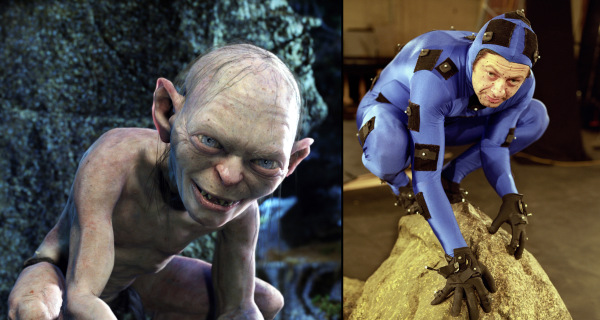
\includegraphics[width=\textwidth]{img/gollum}
                \caption{Golum in Lord of the Rings (Image from New Line Cinema)}
        \end{subfigure}
        \begin{subfigure}[t]{0.43\textwidth}
                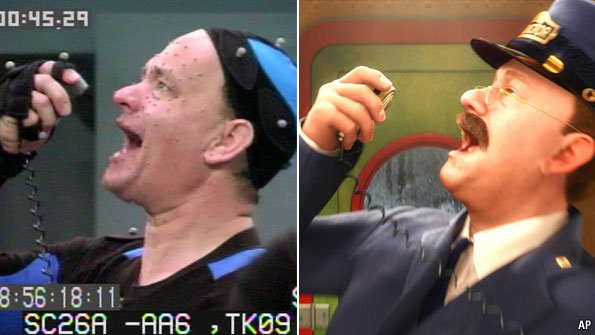
\includegraphics[width=\textwidth]{img/polar_express}
                \caption{Train conductor in Polar Express (Image from Warner Bros.)}
        \end{subfigure}
        \caption{Motion capture examples in the VFX industry.}
        \label{fig:results1}
\end{figure}

In the last two decades, nearly two hundred academic papers that include words \textit{face}, \textit{animation} and \textit{motion capture} were published in computer graphics and vision journals ~\cite{Scopus}. The increase in the quality of the results is explained by the advancements in both the capturing technology and the computational methods. We shall concentrate on the latter; for a brief discussion of the capturing methods see Sec.~\ref{sec:datacapture}. 

The work of Guenter et al. provides the first detailed and unified system for capturing and reconstructing facial performance~\cite{Guenter:1998}. Their work is mostly focused on motion tracking and production of labelled three-dimensional motion of the dots on the actor's face. Once a sequence of  moving dots is acquired, the author's face is scanned to obtain a polygonal mesh that corresponds to the geometry of the face. The motion of the sparse dots is described in terms of offsets from the neutral position. Then the vertices in the mesh are moved by calculating a linear combination of the offsets of the nearest dots, i.e. in each frame a weighted sum of the change in the dot position is calculated and added to the neutral position of the given vertex. The weights are chosen to be zero everywhere except in the one-ring neighbourhood where the weights depend on the distance of the vertex to the dots; the weights must sum to one. An additional stationary ring of dots is added on the edge of the face to ensure there is no motion outside the face. The algorithm suffers from noise introduced during in the tracking, the reconstruction and the three-dimensional scanning. Moreover, the choice of the nearest dots for each vertex in the mesh is not trivial due to the irregular distribution of the tracked dots. The method that assigns the blends has a number of manually adjusted parameters and does not guarantee to find the best set of reference dots. Additionally, the areas around the eyes and lips require a special treatment; the dots above and below the problematic areas are marked and are not allowed to be blended. The authors point out that a number of artefacts are visible in the resulting animation; some of these flaws are attributed to the poor quality of the facial scan, the fact that the reconstruction method is not robust to jitter and incorrect placement of the tracked data.

At around the same time Pinghin et al. proposed a method for synthesizing facial expressions form photographs~\cite{Pighin:1998}. The authors concentrate their attention on the capture and reconstruction part of the process. First, a three-dimensional model of the face pulling a number of different expressions is constructed, then the animation is created by morphing these meshes and producing the intermediate motion. The meshes are topologically consistent and the features are marked manually, resulting in matching feature sets. Then linear interpolation between corresponding vertices in the different meshes is used to get a smooth morphing. Compared to the method proposed by Guenter et al., the approach of Pinghin et al. puts more emphasis on the capture, reconstruction, and creation of good quality meshes for different expressions resulting in an almost trivial animation production process.

Noh and Neumann addressed the problem of having to create a new model for a new animation by exploiting an existing database of high quality animations~\cite{Noh:2001}. Given a new target model, dense correspondence between the source model from the database and the target is estimated using a set of manually selected matching points. The volume morphing is performed using a weighted linear combination of Radial Basis Functions (RBF). However, some manual input is required when matching the features; for this authors employ a set of heuristic rules. Then a cylindrical projection is used to transfer the vertices from the source onto the target model, thus the source vertices are embedded in the target surface. The animation is created by applying the adjusted target motion vector to the source. The adjustments involve scaling, and change of direction according to the curvature of the source surface. Moreover, if the two models have very different geometries, then small neighbourhoods are used to determine the local changes that were imposed during the morphing of the source surface. As in most facial models, special attention is paid to the area around the mouth; the edges of the lips in the two models are aligned, and the motion transformations take into account the motion of both lips to ensure that the duplicated vertices move consistently. The presented approach has a number of limitations; the model requires manual matching, the eyelids, the teeth and the tongue are not incorporated in the model, and it is only able to reproduce the motion of the source model and cannot produce novel movements. 

Building on previous work on synthesis of facial expressions, by Joshi et al. address the problem of automating the creation of blendshapes~\cite{Joshi:2003}. The proposed method segments the face into characteristic parts that can then be modified independently to make a desired expression thus simplifying the process of creating new blendshapes. The authors argue that one of the advantages of controlling small regions is the increased number of expressions that may be produced using the blendshapes. Each frame in the keyframe animation is produced by calculating the linear combination of blendshapes in each region. A linear elasticity model is used to deform the surfaces. A related method,  proposed by Pyun et al. generates a new facial expression by combining emotional and verbal key expressions~\cite{Pyun:2003}. The main limitation of this model is that a set of key expressions have to be designed by an artist. 

In some situations the sets of blendshapes is only available for the target model. Choe and Ko propose a method that constructs a set of source key shapes given the target key shapes~\cite{Choe:2005}. First, a mapping between the source and the target coordinate systems is constructed. Then the method iteratively refines the set of shapes using the captured source data. The authors build on their previous work, and use a muscle actuation basis as opposed to the surface-based key shapes. The elements in the actuation basis are linearly independent and they span the corresponding space, forming a complete basis for the facial expressions~\cite{Choe:2001}. However, the actuation basis is much harder to construct in comparison to the surface-based  set of shapes and the relation between the motion of facial muscles and the resulting motion of the facial tissue is not straight-forward.

Vlasic et al. proposed an novel approach to facial animation that is based on a multilinear model~\cite{Vlasic:2005}. The work offers an alternative approach to blendshape models; it involves creating a large dataset that encodes various features, for instance the identities, expressions and location of vertices. Each dimension of the data tensor corresponds to a unique feature, and due to the independence of modes, each feature may be varied without affecting the others. Such model can be extended to include an arbitrary number of features, and may be used for motion retargeting or actor replacement, when a database of three-dimensional scans is available. Moreover, the probabilistic interpretation of the model is related to probabilistic principal component analysis, and is able to deal with missing data. 

A number of dimensionality reduction techniques have been used to produce facial animation; for example Blanz and Vetter apply principal component analysis (PCA) to create a controllable low dimensional model~\cite{Blanz:1999}. Deng et al. use PCA to find a correspondence between the motion capture data are the manually tuned blendshape model~\cite{Deng:2006}. An extension to nonlinear dimensionality reduction techniques was presented by Wang et al.~\cite{Wang:2004}. The proposed method separates the time-varying facial expressions and the individual style associated with the performer. Then the locally linear embedding (LLE) framework is used to find a nonlinear mapping from the high dimensional space onto a low dimensional manifold. The LLE method is based on an assumption that small neighbourhoods around each data point may be treated as linear patches. Using the resulting generative model, new expressions or an animation may be produced by sampling from the low dimensional manifold.
Dimensionality reduction is used when no blendshape model is available, or when different features of the data need to be extracted.

Most of the previously described methods are unable to capture and reproduce the fine details on the actor's face; Bicket et al. introduced a method that is able to create detailed wrinkles on the target model~\cite{Bickel:2007}. The approach is based on decomposition of the model into coarse features from the motion capture sequence, and fine features from the accompanying video. The novel part of their method relies on capturing, analysing and reproducing the wrinkled surface. In the tracking stage, uniform B-Splines are fitted to each fold of the skin. Then the shape of each fold is estimated by exploiting the self-shadowing effect, and finding the gradient that describes the shape of each fold. Moreover, the coupling behaviour is modelled separately. New wrinkles are synthesised by minimising the associated non-linear shell energy; the geometrical model, proposed by Grinspun et al. estimates the local curvature of a surface, and is able to capture the behaviour of thin flexible structures~\cite{Grinspun:2003}. The facial model with detailed wrinkles relies on the quality of the captured data; in particular, the areas that are prone to small-scale deformations have to be painted in a way that minimises diffuse reflection.

One of the most successful attempts to produce a photo-realistic facial animation is known as the Digital Emily project~\cite{Alexander:2009}. The proposed pipeline involves collecting high resolution data, building a detailed facial rig of the actor's face, producing an animation from the video data, and reproducing the high quality results. The blendshape model was created using approximately $30$ three-dimensional scans; since each scan contained more than one discrete shape, a splitting algorithm had to be used to obtain a larger set of controllable shapes. Additional subtle effects, such as the motion of the deformation of the eyelid when the eyes are closed were included to increase the realism of the results. The animation is produced using a number of example poses, and generating predictions for the required pose of the digital model. The entire production process is very time consuming and requires manual input from skilful artists and animators. The authors do not provide a detailed description of the method but their controllable facial rig is publicly available.

One recent development was proposed by Bouaziz et al., who develop a method for real-time facial animation~\cite{Bouaziz:2013}. The new method does not rely on the construction of a three-dimensional expression model  associated with the actor prior to the face animation stage. The presented method uses a consumer-level device that captures both the intensity and the depth (RGB-D cameras); previous research by Baltru\v{s}aitis et al. indicates that the use of multimodal data improves the quality of feature tracking~\cite{Baltrusaitis:2012}. To achieve real-time results, Bouaziz et al. use a template blendshape model that is constantly updated to better match the face of the performer. This update includes two steps. Firstly, PCA is used to construct a low dimensional representation of a large set of different facial meshes, then any new face is constructed by merging the average face with a linear combination of the orthonormal basis vectors produced by PCA. Secondly, surface deformation field is used to further refine the blendshape model. Then the tracking, retargeting and production of an animation is performed in parallel with the optimisation algorithm that aims to personalise the blendshape model. 

Concurrently, Li et al. combined blendshape models with facial tracking to animate a target character face~\cite{Li:2013}. The authors employ per frame correctives to achieve run time shape correction. The data is captured using RGB-D cameras. The initial state of this method consists of capturing a three-dimensional model of an actor's face, and PCA  and a large database of captured facial data is used to construct a generic face. A blendshape model is constructed using the deformation transfer algorithm, proposed by Sumner and Popovi\'{c}~\cite{Sumner:2004}. Then the motion is produced using blendshapes, and it is refined using an orthogonal adaptive basis. This basis is constructed using PCA, and it contains the initial blendshapes as well as a set of corrective shapes; these additional basis elements correspond to expressions that are not contained in the original shape set. The corrective shapes capture the fine-scale details. Due to the non-linear nature of the resulting blendshape model, Laplacian deformations are used to align the tracked data to the three-dimensional model. Then the expectation-maximisation algorithm is used in the adaptive PCA space to iterative improve the space of the corrective shapes. Specifically, given a number of sufficiently diverse input samples and the initial guess of the corrective space, the algorithm estimates the coefficients of the corrective space. Then, the algorithm finds the model that best explains the samples given the corrective coefficients. After each two cycles of the algorithm, the newly acquired corrective space is orthonormalised, and used to decrease the error during the tracking. This method is capable of producing appealing visual results in real-time. However, it requires a scan of the actors face, and the corrective shapes are not directly used during the retargeting.

A different direction was chosen by Garrido et al., who aim to reconstruct high quality three-dimensional models using data only from a monocular video~\cite{Garrido:2013}. The method relies on a pre-designed blendshape model, and uses optical flow to produce three-dimensional motion. Meanwhile, Xu et al. improved the retargeting of facial animation from an actor onto a digital model~\cite{Xu:2014}. The authors use a multi-scale approach, where a targeted optimisation algorithm is used to achieve best results at the course and the fine scale. Moreover, the proposed method provides the user with a set of control tools that are used to alter the automatically produced results. This blendshape model produces high-quality visual results but it still requires significant input from the user.

%there exist a trade-off between the effort 

%-----------------------------------------------------------------------
\section{Skin Rendering}

Rendering realistic skin is a challenging task.
As social beings we interact with interact with other individuals on a daily basis, which has made human perception quite sensitive to skin appearance, even more so with human faces.
Skin is composed of several layers with different properties, to accurately simulate skin the light transport between this layers has to be simulated.
The full effect of light scattering between two points on the surface can be modelled using a Bidirectional Surface-Scattering Distribution Function (BSSRDF).

Weyrich et al~\cite{Weyrich2006} proposed a two-layer model for skin rendering, the outer layer simulates the air-oil interface and the inner layer models the subsurface scattering in the skin.
The authors considered the scattering to be homogeneous, with this assumption they measured the skin BRDF of several subjects in a light dome, while the scattering was sampled at three points in the face with a custom made sensor.
The BRDF data was fitted to a Blinn-Phong and a Torrance-Sparrow isotropic models, and the scattering was fitted with a single transport coefficient.
Donner et al~\cite{Donner2008} also proposed a two-layer model, however the authors allow for the layers to be heterogeneous.
With this addition they are able to introduce the effects of haemoglobin, veins and tattoos.
Emotional induced haemoglobin variations have also been explored ~\cite{Jimenez2010}.
The authors measured the haemoglobin distributions of several subjects in different poses, then a linear combination of the captured data would determine the final haemoglobin distribution for a new sequence.
Recently, Iglesias et al~\cite{Iglesias2015} introduced a five-layer model to handle skin ageing.
Haemoglobin, collagen and fat changes with age are modelled using the different layers.

Normal maps are use to alter the normals of the scene objects during rendering.
This technique is used to add geometric detail to an object at rendering time without actually changing the geometry.
%The error introduced with this approach is shown in Figure \ref{fig:normal_map}, a ray $r_1$ hist the geometry at point $p$ and the normal $n_p$ is used for shading, while if we had the based geometry the hitting point would be $p'$ and the normal $n'$.
Normal maps for skin rendering are usually captured using expensive light domes with a number of synchronized cameras ~\cite{Graham2013, Weyrich2006}. 

Another technique to increase the quality of a face render is to scale the resolution of the textures being used.
According to cite{Tian2011} super-resolution techniques can be classified into four classes: \textit{frequency-domain}-based,	\textit{interpolation}-based, \textit{regularization}-based and \textit{learning }-based.

\textit{Frequency-domain}-based super-resolution methods started with the seminal work of ~\cite{Tsai:1984}, the authors transformed the image using the discrete Fourier transform, where it is possible to formulate a system of equations relating the discrete and the continuous Fourier transform coefficients.
The system is solved, the new coefficients are apply in the Fourier domain and a new image of higher resolution is retrieved by performing the inverse transformation.
More recently, extensions that include denoising stages \cite{Chappalli:2005} or error handling for registration and blur identification \cite{Ji:2009} has been proposed.

\textit{Interpolation}-based approaches used the fact that if we have several low-resolution images of a scene, each of them provides an amount of additional information about the scene.
This technique projects all the low-resolution images into the hight resolution space and fuses the data maximizing the quality.
Bose et al.~\cite{Bose:2006} proposed a fusing technique using the moving least square (MLS) method, the authors estimated the pixel value as a polynomial approximation of the pixel neighbourhood with adaptive polynomial order for each pixel.
Takeda et al.~\cite{Takeda:2007} proposed a method to generalize this and other problems such as denoising or interpolation into a generalized kernel regression problem.

\textit{Regularization}-based methods tackle the problem from a probabilistic viewpoint.
An estimation using the maximum likelihood (ML) of the high-resolution image $\mathbf{X}^{ML}$ was proposed by Tom et al.~\cite{Tom:1995}, such that

\begin{equation}
\mathbf{X}^{ML} = \underset{\mathbf{X}}{\argmax} P(\mathbf{Y} | \mathbf{X}),
\end{equation} 

where $\mathbf{Y}$ the unknown high-resolution image and $\mathbf{X}$ is the low resolution image.
Extensions using maximum a posterior (MAP) with Markov random fields ~\cite{Humblot:2006} and Markov Chain Monte Carlo methods ~\cite{Tian:2010} have been researched.

In the \textit{learning}-based area, Wie et al.~\cite{Wei:2000} proposed a technique to synthesized new textures based on a sample image and a random noise.
The main idea of the authors work was to maximize the local similarity when choosing a new pixel in the synthesized texture image, based on the already built neighbourhood in the new image.
Ashikhmin et al.~\cite{Ashikhmin2001} presented a method to generate new textures using a goal image by greedily extending existing patches whenever possible.
Hertzmann et al.~\cite{Hertzmann2001} combined and extended Ashikhmin et al.~\cite{Ashikhmin2001} and Wie et al.~\cite{Wei:2000} methods by adding a second example image and using more complex distance metric to choose the next synthesized pixel.
Graham et al.~\cite{Graham2013} applied Hertzmann et al.~\cite{Hertzmann2001} example-based filter to generate bump maps with increased quality for skin rendering.
An alternative approach using a dictionary of samples was presented by Jianchao et al.~\cite{Jianchao2010}.
This method is restricted to generating super-resolution images, however, the previous methods support a wide variety of filter effects.
For an in depth analysis of super-resolution techniques, we refer the readers to Tian et al.~\cite{Tian2011} survey.

%\begin{figure}[htbp!]
%\centering
%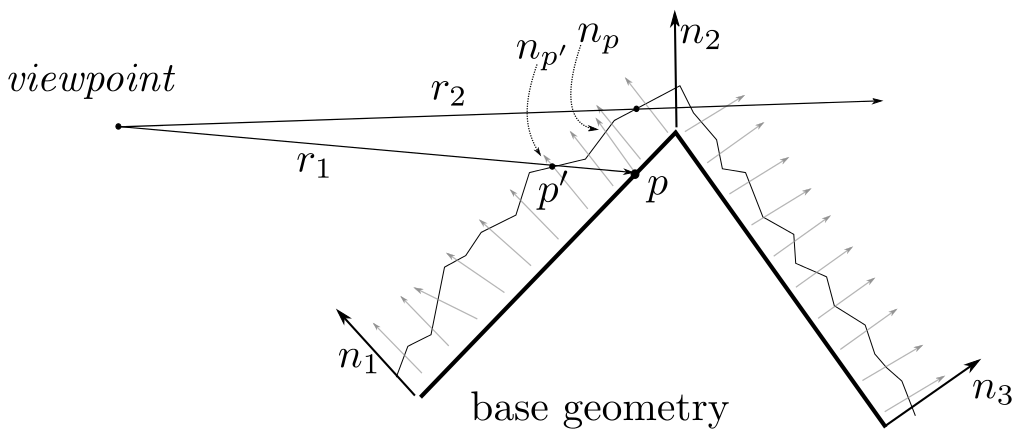
\includegraphics[width=0.7\textwidth]{img/normal_map}
%	\caption{ Using normal maps to simplify a given geometry, image taken from \cite{ganovelli2014}.}
%	\label{fig:normal_map}
%\end{figure}